\documentclass[11pt]{article}
\usepackage[utf8]{inputenc}
\usepackage[T1]{fontenc}
\usepackage{amsmath}
\usepackage{amssymb} % Needed for \eth
\usepackage{graphicx}
\usepackage{geometry}
\usepackage{tikz}
\usepackage{pgfplots} % For plots
\usepackage{ulem}     % For underline, using normalem to avoid messing with \emph
\usepackage{tcolorbox} % For boxing equations
\usepackage{braket}    % For QM state notation if needed

\geometry{a4paper, margin=1in}
\usetikzlibrary{positioning, arrows.meta, shapes.geometric, patterns, calc} % Added calc library
\pgfplotsset{compat=1.18} % Use a recent PGFPlots version

% Custom commands (optional)
\newcommand{\avg}[1]{\overline{#1}}
\newcommand{\prob}[1]{P(#1)}
\newcommand{\ProbDens}[1]{\mathcal{P}(#1)} % Using script P for density
\newcommand{\vect}[1]{\vec{#1}}
\newcommand{\dd}[1]{\mathrm{d}#1} % Differential d
\newcommand{\pderiv}[2]{\frac{\partial #1}{\partial #2}}
\newcommand{\deriv}[2]{\frac{\mathrm{d} #1}{\mathrm{d} #2}}
\newcommand{\muState}{\mu\text{-state}} % Microstate
\newcommand{\OmegaE}{\Omega(E)}
\newcommand{\omegaE}{\omega(E)}
\newcommand{\PhiE}{\Phi(E)}
\newcommand{\deltaE}{\delta E}
\newcommand{\ethbar}{\text{\it{đ}}} % \eth symbol for inexact differential
\newcommand{\kb}{k_B} % Boltzmann constant
\newcommand{\gasR}{R} % Ideal gas constant
\newcommand{\partfn}{Z} % Partition function symbol
\newcommand{\grandpartfn}{\mathcal{Z}} % Grand partition function symbol
\newcommand{\lambdaT}{\lambda_{th}} % Thermal wavelength
\newcommand{\muB}{\mu_B} % Bohr Magneton
\newcommand{\Na}{\mathrm{N_A}}

% Define a tcolorbox style for boxed equations
\tcbuselibrary{skins}
\newtcolorbox{eqbox}[1][]{
  enhanced,
  colback=yellow!10!white,
  colframe=blue!75!black,
  boxrule=1pt,
  arc=3mm,
  #1
}

\title{Physics 415 - Lecture 24: Specific Heat of Solids, Paramagnetism}
\date{March 17, 2025}
\author{} % Author not specified

\begin{document}

\maketitle
\thispagestyle{empty}

\section*{Summary}

\begin{itemize}
    \item Classical Partition Function (N identical particles):
    \[ \partfn = \frac{1}{N!} \int \prod_{i=1}^N \frac{d^3 q_i d^3 p_i}{(2\pi\hbar)^3} e^{-\beta E(q,p)} \]
    where $E(q,p) = K(p) + U(q)$.
    \item Equipartition Theorem (Classical): Each quadratic term in $E$ contributes $\frac{1}{2}T$ (or $\frac{1}{2}\kb T$) to $\avg{E}$.
    \item Quantum Harmonic Oscillator ($E_n = (n+1/2)\hbar\omega$):
    \[ \partfn = \frac{e^{-\beta\hbar\omega/2}}{1-e^{-\beta\hbar\omega}}, \quad \avg{E} = \hbar\omega \left( \frac{1}{2} + \frac{1}{e^{\beta\hbar\omega}-1} \right) \]
\end{itemize}

\section*{Specific Heat of Solids}

An important application of the quantum harmonic oscillator results and the classical equipartition theorem is to the specific heat of solids.

Consider a simple solid with one atom type ($N$ atoms total) in the unit cell (e.g., elemental metal like Cu, or diamond). The atoms vibrate about their equilibrium lattice positions. These are "lattice vibrations".
The system can be described as $N$ coupled 3D harmonic oscillators. By transforming to normal mode coordinates $(q_i, p_i)$, the Hamiltonian can be written (approximately) as a sum of $3N$ independent 1D harmonic oscillators:
\[ E = \sum_{i=1}^{3N} \left( \frac{p_i^2}{2m_i^*} + \frac{1}{2} m_i^* \omega_i^2 q_i^2 \right) \]
where $\omega_i$ are the normal mode frequencies and $m_i^*$ are effective masses.

\subsection*{High Temperature Limit (Classical)}

At high temperatures, $T \gg \hbar\omega_{max}$ (where $\omega_{max}$ is the maximum normal mode frequency), we expect a classical treatment to be valid.
The Hamiltonian has $3N$ quadratic momentum terms and $3N$ quadratic position terms, for a total of $6N$ quadratic degrees of freedom.
By the classical equipartition theorem:
\[ \avg{E} = 6N \times (\frac{1}{2}T) = 3NT \]
(Using $T$ in energy units, $k_B=1$). Or using $T$ in Kelvin: $\avg{E} = 3N \kb T$.
In terms of moles ($N = \nu \Na, \gasR = \Na \kb$):
\[ \avg{E} = 3 \nu \gasR T \]
The heat capacity at constant volume is:
\[ C_V = \left( \pderiv{\avg{E}}{T} \right)_V = 3N \kb = 3 \nu \gasR \]
The molar specific heat is:
\[ c_v = \frac{C_V}{\nu} = 3 \gasR \]
This is the \textbf{Dulong-Petit Law}: At high enough temperatures, the molar specific heat of simple solids is approximately $3R \approx 25$ J/(mol·K).

\subsection*{Low Temperature Correction (Quantum)}

At lower temperatures, we must use the quantum result for the average energy of harmonic oscillators.
\[ \avg{E} = \sum_{i=1}^{3N} \hbar\omega_i \left( \frac{1}{2} + \frac{1}{e^{\beta\hbar\omega_i}-1} \right) \]
To evaluate the sum, we need to know the distribution of normal mode frequencies $\omega_i$, known as the phonon density of states.

\textbf{Einstein Model (1907):} A crude approximation assumes all normal modes have the same frequency, $\omega_i = \omega_E$. Define the Einstein temperature $\theta_E = \hbar\omega_E / \kb$.
\[ \avg{E} = 3N \hbar\omega_E \left( \frac{1}{2} + \frac{1}{e^{\beta\hbar\omega_E}-1} \right) = 3N \kb \theta_E \left( \frac{1}{2} + \frac{1}{e^{\theta_E/T}-1} \right) \]
The heat capacity is $C_V = (\partial \avg{E} / \partial T)_V$.
\[ C_V = 3N \kb \left( \frac{\theta_E}{T} \right)^2 \frac{e^{\theta_E/T}}{(e^{\theta_E/T}-1)^2} \]
The molar specific heat is $c_v = C_V / \nu = 3\gasR (\frac{\theta_E}{T})^2 \frac{e^{\theta_E/T}}{(e^{\theta_E/T}-1)^2}$.

\textbf{Limits:}
\begin{itemize}
    \item High T ($T \gg \theta_E$): Let $x = \theta_E/T \ll 1$. $e^x \approx 1+x$.
    $c_v \approx 3\gasR x^2 e^x / (e^x-1)^2 \approx 3\gasR x^2 (1+x) / ((1+x)-1)^2 = 3\gasR x^2 (1+x) / x^2 \approx 3\gasR$. Recovers Dulong-Petit law. $\checkmark$
    \item Low T ($T \ll \theta_E$): Let $x = \theta_E/T \gg 1$. $e^x \gg 1$.
    $c_v \approx 3\gasR x^2 e^x / (e^x)^2 = 3\gasR x^2 e^{-x} = 3\gasR (\frac{\theta_E}{T})^2 e^{-\theta_E/T}$.
    Predicts strong exponential suppression $c_v \to 0$ as $T \to 0$. $\checkmark$
\end{itemize}

The Einstein model qualitatively captures the decrease of $C_V$ at low T, but the exponential decay is too fast compared to experiments, which typically show $c_v \propto T^3$ at low T. The \textbf{Debye model} uses a more realistic distribution of frequencies and correctly predicts the $T^3$ behavior (details later).

\begin{center}
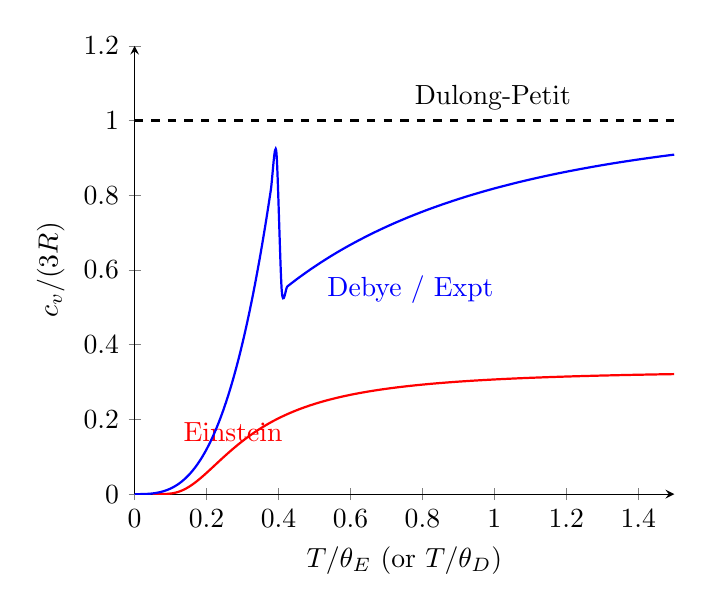
\begin{tikzpicture}
\begin{axis}[
    xlabel={$T / \theta_E$ (or $T/\theta_D$)}, % Use characteristic Temp scale
    ylabel={$c_v / (3R)$},
    xmin=0, xmax=1.5, ymin=0, ymax=1.2,
    axis lines=left,
    legend pos=south east
]
% Dulong-Petit limit
\addplot [domain=0:1.5, dashed, thick, black] {1} node[pos=0.5, anchor=south west] {Dulong-Petit};
% Einstein Model
\addplot [domain=0.05:1.5, samples=100, smooth, thick, red] {(1/x)^2 * exp(1/x) / (exp(1/x)-1)^2 / 3} node[pos=0.3, anchor=north east] {Einstein};
% Debye Model (schematic T^3 rise)
\addplot [domain=0:1.5, samples=100, smooth, thick, blue] { (x<0.4) ? (15*x^3) : (1 - exp(-1.8*x^0.8)*1.1) } node[pos=0.6, anchor=north west] {Debye / Expt}; % Approx T^3 then saturation

\end{axis}
\end{tikzpicture}
\end{center}

\section*{Paramagnetism}

As another application of CE statistical mechanics, consider paramagnetism.
A paramagnet is a material in which a non-zero net magnetic moment is generated along the direction of an applied magnetic field $\vec{H}$.
Paramagnetism is a quantum phenomenon, arising from unpaired electron spins or orbital angular momenta in atoms/ions of the material. We can analyze key properties using stat mech.

Consider a system of $N$ non-interacting atoms (or ions) in a material at temperature $T$, placed in magnetic field $\vec{H}$. Assume each atom has a total angular momentum $\vec{J}$ (quantum number $J = 1/2, 1, 3/2, \dots$).
From QM, the magnetic dipole moment is related to angular momentum:
\[ \vec{\mu} = g \muB \vec{J}/\hbar \]
where $\muB = e\hbar/(2m_e c)$ is the Bohr magneton, and $g$ is the g-factor (Lande g-factor, $\approx 2$ for electron spin).
The magnetic energy of an atom in field $\vec{H}$ (assume $\vec{H}$ along z-axis) is:
\[ \epsilon = -\vec{\mu} \cdot \vec{H} = -(g \muB J_z/\hbar) H \]
From QM, the allowed values of $J_z$ are $m\hbar$ where $m = -J, -J+1, \dots, J-1, J$. There are $(2J+1)$ possible values for $m$.
The energy levels are:
\[ \epsilon_m = -g \muB H m \]

\textbf{Single Atom Partition Function ($Z_1$):}
Consider one such atom in contact with a reservoir at $T$.
\[ Z_1 = \sum_{m=-J}^{J} e^{-\beta \epsilon_m} = \sum_{m=-J}^{J} e^{\beta g \muB H m} \]
Let $\eta = \beta g \muB H = g \muB H / T$.
\[ Z_1 = \sum_{m=-J}^{J} (e^\eta)^m \]
This is a finite geometric series with $r=e^\eta$, first term $a=r^{-J}=(e^\eta)^{-J}$, and $N_{terms}=2J+1$.
Sum $= a (1-r^{N_{terms}}) / (1-r) = e^{-J\eta} (1 - e^{(2J+1)\eta}) / (1-e^\eta)$.
\[ Z_1 = \frac{e^{-J\eta} - e^{(J+1)\eta}}{1 - e^\eta} \]
Multiply numerator and denominator by $e^{-\eta/2}$:
\[ Z_1 = \frac{e^{-(J+1/2)\eta} - e^{(J+1/2)\eta}}{e^{-\eta/2} - e^{\eta/2}} = \frac{-2 \sinh((J+1/2)\eta)}{-2 \sinh(\eta/2)} \]
\[ Z_1 = \frac{\sinh((J+1/2)\eta)}{\sinh(\eta/2)} \]

\textbf{Average Magnetic Moment:}
The z-component of the magnetic moment for state $m$ is $\mu_{z,m} = g \muB m$.
The average magnetic moment is $\avg{\mu_z} = \sum_{m=-J}^J P_m \mu_{z,m}$.
\[ \avg{\mu_z} = \sum_{m=-J}^J \frac{e^{-\beta \epsilon_m}}{Z_1} (g \muB m) = \frac{g \muB}{Z_1} \sum_{m=-J}^J m e^{\beta g \muB H m} \]
Use the relation $\avg{O} = (1/\beta) \partial(\ln Z)/\partial X$ if $E = E_0 - O X$. Here $E = 0 - \mu_z H$, so $O = \mu_z$.
$\avg{\mu_z} = (1/\beta) \partial(\ln Z_1)/\partial H$.
\[ \avg{\mu_z} = T \pderiv{(\ln Z_1)}{H} = T \pderiv{\eta}{H} \pderiv{(\ln Z_1)}{\eta} \]
Since $\eta = g\muB H / T$, $\partial \eta / \partial H = g \muB / T$.
\[ \avg{\mu_z} = T \left( \frac{g \muB}{T} \right) \pderiv{(\ln Z_1)}{\eta} = g \muB \pderiv{(\ln Z_1)}{\eta} \]
$\ln Z_1 = \ln \sinh((J+1/2)\eta) - \ln \sinh(\eta/2)$.
\[ \pderiv{(\ln Z_1)}{\eta} = (J+1/2) \frac{\cosh((J+1/2)\eta)}{\sinh((J+1/2)\eta)} - (1/2) \frac{\cosh(\eta/2)}{\sinh(\eta/2)} \]
\[ \pderiv{(\ln Z_1)}{\eta} = (J+1/2) \coth((J+1/2)\eta) - (1/2) \coth(\eta/2) \]
This expression defines the Brillouin function $B_J(x)$ where $x=J\eta$:
\[ B_J(x) = \frac{1}{J} \left[ (J+1/2) \coth((J+1/2)\frac{x}{J}) - (1/2) \coth(\frac{x}{2J}) \right] \]
Then:
\[ \avg{\mu_z} = g \muB J B_J(J\eta) = g \muB J B_J( \beta g \muB H J ) \]
(Note: Source defines $B_J(\eta)$ slightly differently, leading to $\avg{\mu_z}=g\muB J B_J(\eta)$). Let's use the source's implicit definition $\overline{\mu_z}/(g\mu_B) = (J+1/2) \coth[(J+1/2)\eta] - (1/2)\coth(\eta/2)$.

\textbf{Magnetization:}
If there are $n$ atoms per unit volume, the magnetization $M_z$ is:
\[ M_z = n \avg{\mu_z} = n g \muB \left[ (J+1/2) \coth((J+1/2)\eta) - (1/2) \coth(\eta/2) \right] \]
The magnetization is determined by the single parameter $\eta = g\muB H / T$.

\textbf{Limits:}
\begin{itemize}
    \item High T / Low H ($\eta \ll 1$): Use $\coth y \approx 1/y + y/3$ for $y \ll 1$.
    Let $y_1 = (J+1/2)\eta$ and $y_2 = \eta/2$.
    $\avg{\mu_z} / (g\muB) \approx [ (J+1/2) (\frac{1}{y_1} + \frac{y_1}{3}) - (1/2) (\frac{1}{y_2} + \frac{y_2}{3}) ]$
    $\approx [ (J+1/2)\frac{1}{(J+1/2)\eta} + \frac{(J+1/2)^2 \eta}{3} - (1/2)\frac{1}{\eta/2} - \frac{(1/2)^2 \eta}{3 \times 2} ]$
    $\approx [ \frac{1}{\eta} + \frac{(J+1/2)^2 \eta}{3} - \frac{1}{\eta} - \frac{\eta}{12} ] = \frac{\eta}{3} [(J+1/2)^2 - 1/4]$
    $= \frac{\eta}{3} [J^2 + J + 1/4 - 1/4] = \frac{J(J+1)}{3} \eta$.
    $\avg{\mu_z} \approx g \muB \frac{J(J+1)}{3} \eta = g \muB \frac{J(J+1)}{3} \frac{g\muB H}{T}$.
    $M_z = n \frac{(g\muB)^2 J(J+1)}{3T} H$.
    This is $M_z = \chi H$ with susceptibility $\chi = n \frac{\mu_{eff}^2}{3T}$, where $\mu_{eff}^2 = (g\muB)^2 J(J+1)$. This is Curie's Law ($\chi \propto 1/T$).

    \item Low T / High H ($\eta \gg 1$): Use $\coth y \approx 1$ for $y \gg 1$.
    $\avg{\mu_z} / (g\muB) \approx (J+1/2)(1) - (1/2)(1) = J$.
    $\avg{\mu_z} \approx g \muB J$. This is the maximum possible moment (saturation).
    $M_z \approx n g \muB J$. Magnetization saturates, independent of $H$.
\end{itemize}

Plot of $M_z$ vs $\eta$ (Brillouin function shape):
\begin{center}
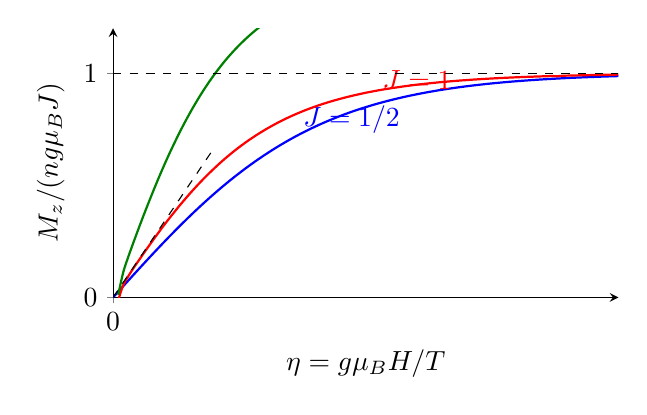
\begin{tikzpicture}
\begin{axis}[
    xlabel={$\eta = g\muB H / T$}, ylabel={$M_z / (n g \muB J)$},
    xmin=0, xmax=5, ymin=0, ymax=1.2,
    xtick={0}, ytick={0, 1},
    axis lines=left, width=8cm, height=5cm,
    legend pos=south east
]
% Brillouin functions B_J(J*eta) / J
% J=1/2: tanh(x/2) / (1/2) = 2 tanh(x/2)? No, avg/(g muB) = J B_J(J eta). avg/(g muB J) = B_J(J eta).
% J=1/2: avg/(g muB) = (1/2) tanh(eta/2).  avg/(g muB J) = tanh(eta/2).
\addplot [domain=0:5, samples=100, smooth, thick, blue] {tanh(x/2)} node[pos=0.6, anchor=north east] {$J=1/2$};
% J=1: avg/(g muB) = (3/2)coth(3eta/2) - (1/2)coth(eta/2). avg/(g muB J) = ...
\addplot [domain=0:5, samples=100, smooth, thick, red] { 1.5/tanh(1.5*x) - 0.5/tanh(0.5*x) } node[pos=0.7, anchor=east] {$J=1$}; % Check formula: Brillouin directly is simpler maybe?
% B_J(x) = ( (2J+1)/(2J) )/tanh((2J+1)x/(2J)) - ( 1/(2J) )/tanh(x/(2J))
% J=1: B_1(x) = (3/2)/tanh(3x/2) - (1/2)/tanh(x/2) -> This is avg/(g muB). Divide by J=1.
\addplot [domain=0:5, samples=100, smooth, thick, green!50!black] { 2/tanh(2*x) - 0.5/tanh(0.5*x) } node[pos=0.8, anchor=east] {$J=3/2$}; % Scaled by 1/J=2/3 ? Let's use limits.

% Saturation
\draw [dashed] (axis cs:0, 1) -- (axis cs:5, 1);
% Linear initial slope
\draw [dashed, domain=0:1] plot (\x, {(1*(1+1)/3)*\x}); % J=1 limit slope (J(J+1)/3)*eta
\end{axis}
\end{tikzpicture}
\end{center}
(See Reif Fig 7.8.3 for comparison between experiment and theory - impressive agreement).

The independent spin approximation generally breaks down at sufficiently low $T$, where interactions between spins cannot be neglected. These interactions can lead to ordered states like ferromagnetism or antiferromagnetism (return to this later).

\end{document}